\begin{savequote}[0.55\linewidth]
  ``The fundamental problem of communication is that of reproducing at one point either exactly or approximately a message selected at another point.''
  \qauthor{Claude Shannon (1916 -- 2001)}
\end{savequote}


%---------------------------------------------------------------------------------- %
% An interesting Chapter
% --------------------------------------------------------------------------------- %
\chapter{An Interesting Chapter} % (fold)
\label{cha:interesting_chapter}
\minitoc

%
% Abstract 
%
In this chapter we overview some general concepts involved in data networks.

\section{Introduction} % (fold)
\label{sec:introduction_to_the_problem}

In the previous chapter, we provided a high-level description of the system following the
great framework proposed in \cite{Bertsekas1992} (note that here we are citing a book, but
we might cite papers as well \cite{Capetanakis1979}). 

The layered architecture is usually modelled according to the Open Systems Interconnection (\acrshort{osi}).

The main layers in the OSI model are typically\footnote{Remember that adding notes for further explanations is never a bad a idea}... 


\subsection{A Subsection} % (fold)
\label{sub:a_subsection}

As shown in Eq. (\ref{eq:srrc_filter})...

\begin{equation}
	g(t) = \sinc(\pi t/ T) \frac{\cos(\pi \beta t/T)} {1 - 4 \beta^2 t^2 / T^2}, 
	\label{eq:srrc_filter}
\end{equation}

\begin{figure}[]
	\centering
	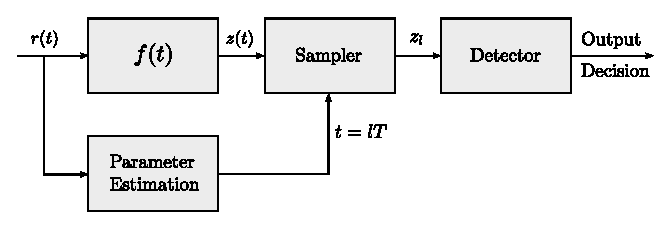
\includegraphics[scale=0.7]{fig/receiver.eps}
	\caption{Receiver architecture.}
	\label{fig:rx_arch}
\end{figure} 

Figure \ref{fig:rx_arch} depicts a simplified receiver architecture that implements the functions described above. 

\section{Summary} 
\label{sec:summary_comm_eng}
In this chapter, some fundamental notions on the design of filters have been addressed.

We showed that: 
\begin{itemize}
	\item maths are great;
	\item filters are linear;
	\item the system is stationary;
\end{itemize}

Thus, our focus in the remaining chapters will be on...

% chapter interesting_chapter (end)